\documentclass[
version=last,toc=bib,toc=graduated,toc=index,toc=listof,9pt,openany]{scrbook}
%\pdfminorversion=4
\usepackage[utf8]{inputenc}
\usepackage[ngerman, english]{babel}
\usepackage{dejavu}

\usepackage{ifmtarg}
\usepackage{ifthen}

\usepackage{geometry}
\geometry{%a6paper
paperwidth=125mm, paperheight=168mm, 
portrait,
top=22mm, inner=22mm, outer=20mm, bottom=25mm,
headsep=3mm, footskip=12mm
}

\usepackage{ragged2e} % schöneren Textsatz (Silbentrennung) bei Nicht-Blocksatz
\usepackage{lscape}
\setlength{\parskip}{0pt}

%\pdfminorversion=4


%\usepackage[babel,german=quotes]{csquotes}
\usepackage{relsize}

\clubpenalty=10000 %keine Schusterjungen
 \widowpenalty=10000 
 \displaywidowpenalty=10000 % keine Hurenkinder

\usepackage[letterspace=16]{microtype} %schönerer Textsatz

\usepackage{graphicx} %Bilder

%Dateipfade, wo die Bilder liegen
\graphicspath{{images-print/}{icons/}{extra-pages/}{wallpaper/}}
\usepackage{wrapfig}  % umflossene Logos von Sponsoren mit Multiabsatztexten

\usepackage{tabu}
\usepackage{tabularx}
\usepackage{longtable}
\usepackage[table,cymk]{xcolor}
\usepackage{colortbl}

% PDF-Seiten einbinden
% pdfpages, darf erst nach colortbl geladen werden!
\usepackage{pdfpages}

% PDFs als Hintergrundbilder
% wallpaper, darf erst nach colortbl geladen werden!
\usepackage{wallpaper}
\usepackage{multirow}
\usepackage{booktabs}
\usepackage{array}

\usepackage{mathabx} % für das Rautensymbol in der Speisekarte
\usepackage{textcomp} % degree symbol

\usepackage{refcount} % Berechnung der Seite, auf der sich die Karte befindet

\usepackage[manualmark]{scrlayer-scrpage}
\pagestyle{scrplain}


\newcommand{\acro}[1]{{\textsmaller{#1}}} % Akronyme

% Überschriften in DejaVu Sans Condensed
\addtokomafont{sectioning}{\fontfamily{DejaVuSansCondensed-TLF}\selectfont}
\addtokomafont{pageheadfoot}{\usefont{T1}{DejaVuSansCondensed-TLF}{m}{n}}
\addtokomafont{pagenumber}{\usefont{T1}{DejaVuSansCondensed-TLF}{m}{n}}


%Titelei
\title{FOSSGIS 2017}
\subtitle{Programm}
\author{FOSSGIS e.V.}
\date{\today}

%\newcommand{\talkroom}{}
\clearscrheadings

% Seitenzahlen
\cfoot[\begin{small}\pagemark\end{small}]{\begin{small}\pagemark\end{small}}
\ofoot[]{}
\ifoot[]{}
\pagestyle{scrplain}

% Durchschuss erhöhen
\linespread{1.15}

% Befehlsdefinitionen einbinden
% neuer Zeitslot
\newcommand{\talktime}{9:99}
\newcommand{\newtimeslot}[1]{\newpage\renewcommand{\talktime}{#1}}

% neuer Zeitslot ohne Seitenumbruch
\newcommand{\newsmalltimeslot}[1]{\renewcommand{\talktime}{#1}}

% \konferenztag initialisieren
\newcommand{\konferenztag}{KeinTag}


% Standard-Seitenstil definieren (Schnittmarken mit Seitenazhl)
\DeclareNewLayer[background, oddorevenpage, width=125mm,%
height=169mm, contents={%
  
\includegraphics{wallpaper/crop-marks.pdf}%
}]{cropmarksevery}
\newpairofpagestyles[scrheadings]{cropmarksstyle}{}
\AddLayersAtBeginOfPageStyle{cropmarksstyle}{cropmarksevery}

% Seitenstil für Titelseite
\DeclareNewLayer[background, oddorevenpage, width=125mm,%
height=169mm, contents={%
  
\includegraphics{wallpaper/deckseite-vektor-mit-schnittmarken.pdf}%
}]{titlelayer}
\newpairofpagestyles[]{titlestyle}{}
\AddLayersAtBeginOfPageStyle{titlestyle}{titlelayer}

% Hintergrund setzen
\def\mittwoch{Mittwoch}
\def\donnerstag{Donnerstag}
\def\freitag{Freitag}

% Seitenstile definieren
% Mittwoch
\DeclareNewLayer[background, oddpage,  width=125mm,%
height=169mm, contents={%
  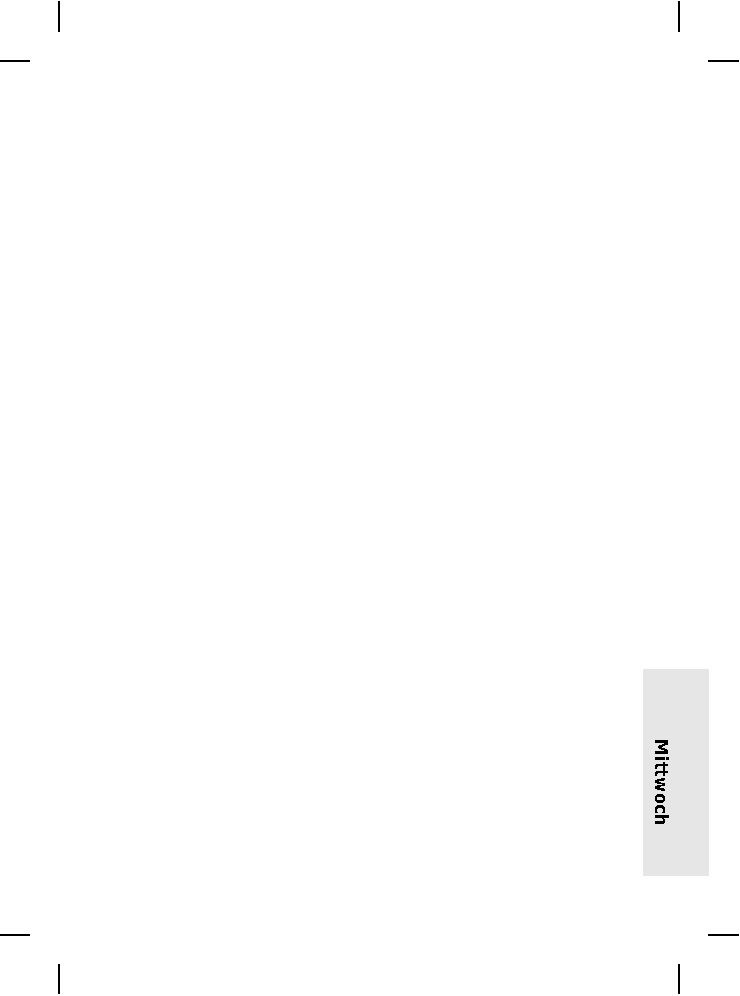
\includegraphics{wallpaper/mittwoch-ungerade.pdf}%
}]{mittwochungerade}
\DeclareNewLayer[background, evenpage,  width=125mm,%
height=169mm, contents={%
  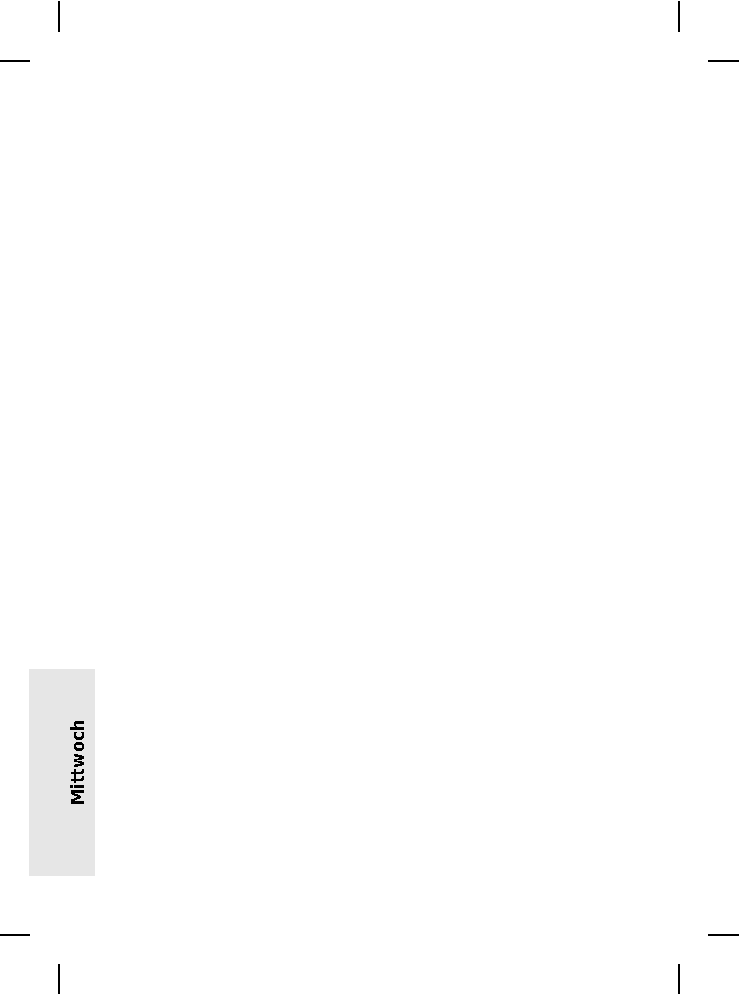
\includegraphics{wallpaper/mittwoch-gerade.pdf}%
}]{mittwochgerade}
\newpairofpagestyles[scrheadings]{mittwoch}{}
\AddLayersAtBeginOfPageStyle{mittwoch}{mittwochgerade}
\AddLayersAtBeginOfPageStyle{mittwoch}{mittwochungerade}
% Donnerstag
\DeclareNewLayer[background, oddpage,  width=125mm,%
height=169mm, contents={%
  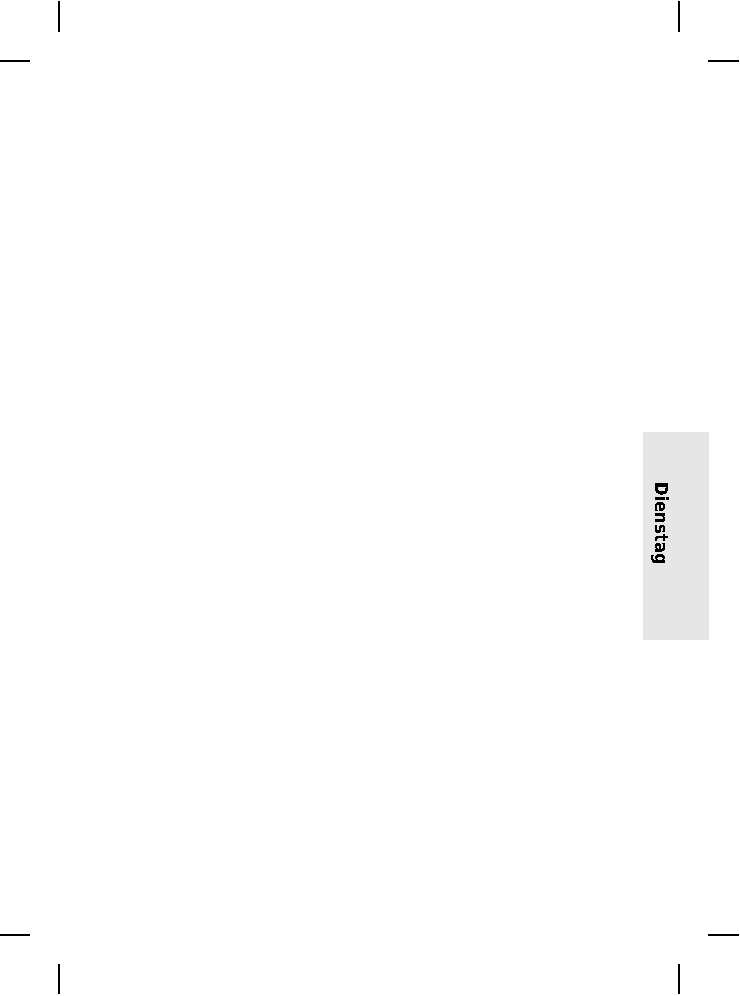
\includegraphics{wallpaper/donnerstag-ungerade.pdf}%
}]{donnerstagungerade}
\DeclareNewLayer[background, evenpage,  width=125mm,%
height=169mm, contents={%
  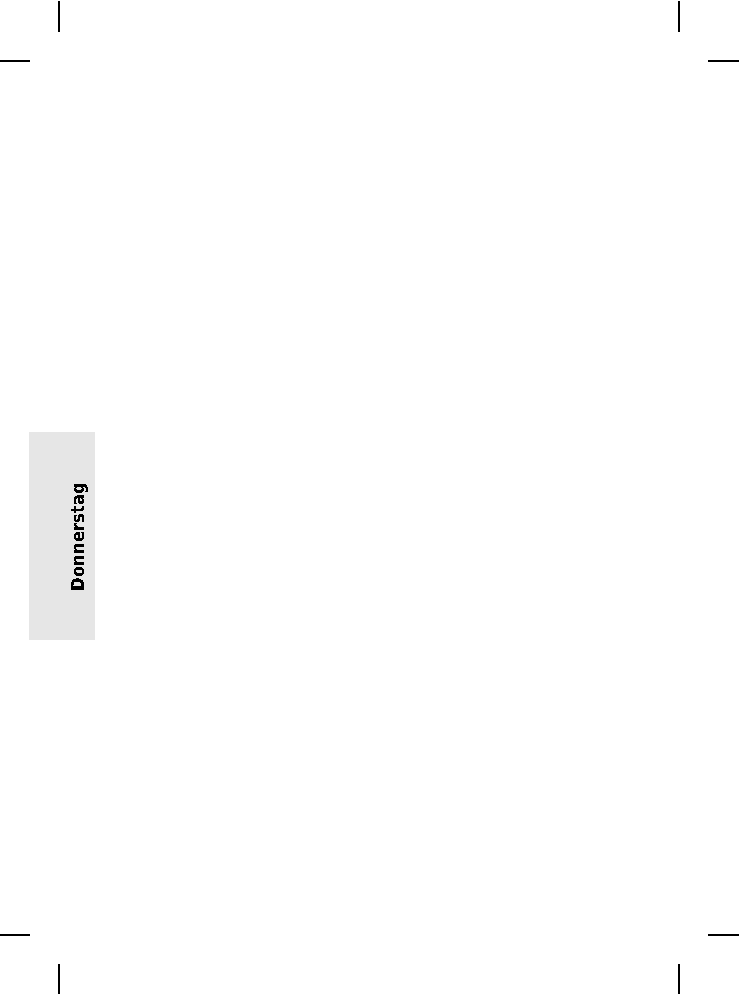
\includegraphics{wallpaper/donnerstag-gerade.pdf}%
}]{donnerstaggerade}
\DeclareNewLayer[background, oddpage,  width=125mm,%
height=169mm, contents={%
  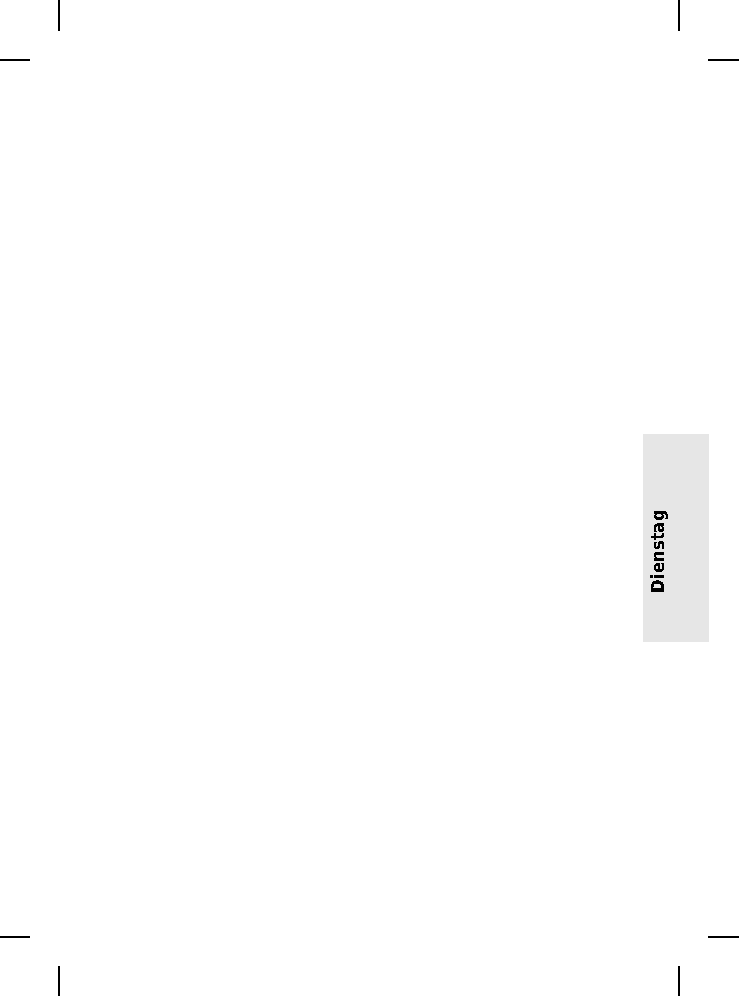
\includegraphics{wallpaper/donnerstag-ungerade-gedreht.pdf}%
}]{donnerstagungeradegedreht}
\newpairofpagestyles[scrheadings]{donnerstag-tabelle}{}
\AddLayersAtBeginOfPageStyle{donnerstag-tabelle}{donnerstaggerade}
\AddLayersAtBeginOfPageStyle{donnerstag-tabelle}{donnerstagungeradegedreht}
\newpairofpagestyles[scrheadings]{donnerstag}{}
\AddLayersAtBeginOfPageStyle{donnerstag}{donnerstaggerade}
\AddLayersAtBeginOfPageStyle{donnerstag}{donnerstagungerade}
% Freitag
\DeclareNewLayer[background, oddpage,  width=125mm,%
height=169mm, contents={%
  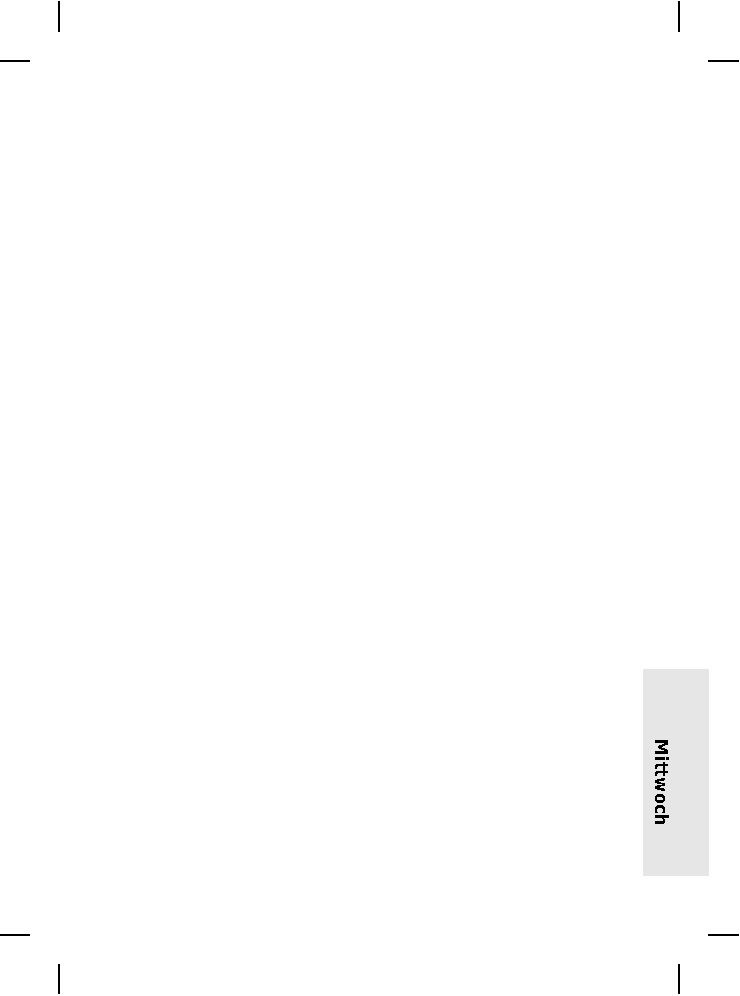
\includegraphics{wallpaper/freitag-ungerade.pdf}%
}]{freitagungerade}
\DeclareNewLayer[background, evenpage,  width=125mm,%
height=169mm, contents={%
  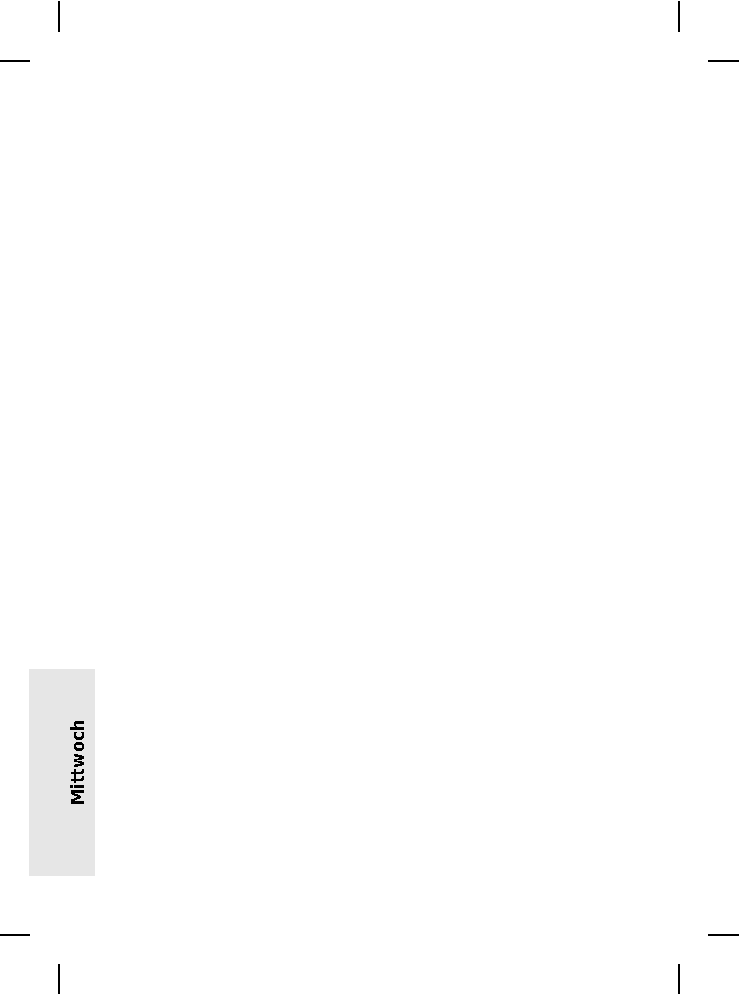
\includegraphics{wallpaper/freitag-gerade.pdf}%
}]{freitaggerade}
\newpairofpagestyles[scrheadings]{freitag}{}
\AddLayersAtBeginOfPageStyle{freitag}{freitaggerade}
\AddLayersAtBeginOfPageStyle{freitag}{freitagungerade}

% \setpagebackground wählt anhand des aktuellen Tages aus, welcher
% Seitenstil verwendet werden soll. Jeder Tag ist ein eigener Seitenstil.
\newcommand{\setpagebackground}{ %
  \ifthenelse{\equal{\konferenztag}{\mittwoch}}{%
    \pagestyle{mittwoch}
  }{}
  \ifthenelse{\equal{\konferenztag}{\donnerstag}}{%
    \pagestyle{donnerstag}
  }{}
  \ifthenelse{\equal{\konferenztag}{\freitag}}{%
    \pagestyle{freitag}
  }{}
}


% zusätzlicher Spaltentyp für die Titeltabelle
\newcolumntype{Y}[1]{>{\RaggedRight\arraybackslash}p{#1}}

%% Längen für Titelboxen
\newlength{\titleboxwidth}
\setlength{\titleboxwidth}{\textwidth}
\advance\titleboxwidth by -6pt

% Befehl zum Setzen von Titelboxen
\newcommand{\setabstract}[6]{
	% 1. Sprecher
	% 2. Titel
	% 3. Untertitel
	% 4. Abstract (Text)
	% 5. Farbe
	% 6. Raum
	%\thispagestyle{scrheadings}
  \setpagebackground
	\setlength\tabcolsep{0pt}
	% \setlength{\fboxsep}{0pt}
	\noindent\fcolorbox{white}{#5}{\parbox{\titleboxwidth}{%
		\noindent\begin{tabu}{X[5L]r}
			\isspeakerempty{#1}{#2}{#6}
			\issubtitleempty{#3}
		\end{tabu}%
	}}
	%
	\isabstractempty{#4}%
	\vspace{0.5em}% Abstand zum nächsten Talk, auch wenn es keinen Abstract gibt
	\setlength\tabcolsep{6pt} % Spaltenpadding wieder auf Default setzen
}

% Setzen des Referenten, falls vorhanden
% Wir gehen davon aus, dass es einen Untertitel nur dann gibt, wenn es auch einen Referenten gibt
\makeatletter
\newcommand{\isspeakerempty}[3]{%
	% Arguments:
	% 1. speaker
	% 2. title
	% 3. room
	\@ifmtarg{#1}{%
			\par\noindent\large \sectfont #2% % Titel
			&
			#3, \talktime
			\tabularnewline
		}
		{
			\emph{#1} % Sprecher
			&
			\talktime
			\tabularnewline
			{\par\noindent\large \sectfont #2}% % Titel
			&
			#3
			\tabularnewline
		}
		
}
\makeatother

% Setzen des Untertitels
% muss ausgelagert und durch \makeatletter umgeben sein
\makeatletter
\newcommand{\issubtitleempty}[1]{%
	\@ifnotmtarg{#1}{\multicolumn{2}{Y{\linewidth}}{\vspace{-0.6em} \noindent\bfseries \normalsize \sectfont #1}\tabularnewline}
}
\makeatother

% Setzen des Abstracts, falls vorhanden
% muss ausgelagert und durch \makeatletter umgeben sein
\makeatletter
\newcommand{\isabstractempty}[1]{%
		\vspace{0.5em}\newline%
		#1 \par% % Abstract
		\vspace{1.5em}% Abstand zum nächsten Talk, auch wenn es einen Abstract gibt
}
\makeatother

% Farben definieren
%\definecolor{eins}{cmyk}{ 0 .18 .06 .10}
\definecolor{eins}{cmyk}{ 0 .13 .04 .08}
\definecolor{zwei}{cmyk}{ .1 0 .17 .05}
\definecolor{hellorange}{cmyk}{ 0 0.13 0.35 0.03}
%\definecolor{aula}{cmyk}{ 0.2 0 0.05 0.13}
\definecolor{aula}{cmyk}{ 0.13 0 0.04 0.11}
\definecolor{geoblau}{cmyk}{ 0.2 .02 0 .01}
\definecolor{dezentrot}{cmyk}{ 0 .17 0.21 .04}
\definecolor{hellgelb}{cmyk}{ 0 .02 0.26 0}
\definecolor{hellgruen}{cmyk}{ 0.05 .0 0.17 0.05}

% Abstract AM HS 9
\newcommand{\abstractNeun}[4]%
{%
	\setabstract{#1}{#2}{#3}{#4}{hellgruen}{AM HS\,9}
}

% Abstract IM HS 13
\newcommand{\abstractDreizehn}[4]%
{%
	\setabstract{#1}{#2}{#3}{#4}{hellgelb}{IM HS\,13}
}

% Abstract IM HS 11
\newcommand{\abstractElf}[4]%
{%
	\setabstract{#1}{#2}{#3}{#4}{geoblau}{IM HS\,11}
}

% Abstract AM HS 10
\newcommand{\abstractZehn}[4]%
{%
	\setabstract{#1}{#2}{#3}{#4}{hellorange}{AM HS\,10}
}

% Workshop STUDLAB
\newcommand{\workshopbox}[3]%
{%
	% 1. Titel
	% 2. Referent
	% 3. HS-Nummer
	\setlength\tabcolsep{0pt}
	\noindent\fcolorbox{white}{dezentrot}{\parbox{\titleboxwidth}{%
			\noindent
			\begin{tabu}{X[5L]r}
				\emph{#2} % Sprecher
				&
				\talktime
				\tabularnewline
				{\noindent\large \bfseries #1}% % Titel
				&
				Workshop #3
				\tabularnewline
			\end{tabu}
		}
	}
	\setlength\tabcolsep{6pt} % Spaltenpadding wieder auf Default setzen
}

% viel zu lang
\newcommand{\zulang}{Dieser Text ist viel zu lang. Dieser Text ist viel zu lang. Dieser Text ist viel zu lang. Dieser Text ist viel zu lang. Dieser Text ist viel zu lang. Dieser Text ist viel zu lang. Dieser Text ist viel zu lang. Dieser Text ist viel zu lang. Dieser Text ist viel zu lang. Dieser Text ist viel zu lang. Dieser Text ist viel zu lang. Dieser Text ist viel zu lang. Dieser Text ist viel zu lang. Dieser Text ist viel zu lang. }

%% Längen für Sponsorenbox
\newlength{\fboxwidth}

\def\workshopsSection{workshopsSection}
\def\abstractsSection{abstractsSection}
\newcommand{\sponsorenbox}[4]{%
  %% Längen für Sponsorenbox
  \setlength{\fboxwidth}{\textwidth}
  \advance\fboxwidth by -7.0pt
  \abstractSponsorenbox{#1}{#2}{#3}{#4}{\workshopsSection}%
}

\newcommand{\sponsorenboxA}[4]{%
  %% Längen für Sponsorenbox
  \setlength{\fboxwidth}{\textwidth}
  \advance\fboxwidth by -10.0pt
  \abstractSponsorenbox{#1}{#2}{#3}{#4}{\abstractsSection}%
}

%% Sponsorenbox
%% 1. Logo
%% 2. Logobreite
%% 3. Anzahl benötigter Zeilen
%% 4. Text
%% 5. Umfeld (\workshopsSection oder \abstractsSection}
\makeatletter
\newcommand{\abstractSponsorenbox}[5]{%
  \setlength{\fboxsep}{4.5pt}%
  \noindent%
  \ifthenelse{\equal{#5}{\workshopsSection}}{%
    \hspace{2.65pt}%
  }{\hspace{-1pt}}%
  \fcolorbox{gray}{white}{\parbox{\fboxwidth}{
    \@ifmtarg{#1}{}{%
      \begin{wrapfigure}[#3]{r}[0pt]{#2}
        \centering\vspace{-1\baselineskip}
        \includegraphics[width=#2]{#1}
      \end{wrapfigure}
    }

    \noindent #4
  }}
  \setlength{\fboxsep}{3pt}
}
\makeatother

% Definitionen für Tagestabellen
\newcolumntype{Z}[1]{>{\RaggedRight\arraybackslash}p{#1}}%
\newcolumntype{C}[1]{>{\Centering\arraybackslash}p{#1}}%
\newcommand{\talk}[2]%
{%
	& \textbf{#1} \newline \emph{#2}
}%
% Titel -- Redner


\newcommand{\workshop}[3]%
{%
	\workshopbox{#1}{#2}{#3}
}%

\newcommand{\otherevent}[1]%
{%
	& \textbf{#1}
}%

\newcommand{\aulaevent}[2]%
{%
	&
	\multicolumn{3}{c}{
		\textbf{#1} (Aula) \par \emph{#2}
	}
}%

\newcommand{\coffeespace}{\vspace{0.4em}}
\newcommand{\workshopspace}{\vspace{0.5em}\\}

% Farben definieren
\definecolor{commongray}{gray}{.9}
%\vspace{-1.2em}
\renewcommand{\arraystretch}{1.4}



\begin{document}
\lsstyle
\usefont{T1}{DejaVuSansCondensed-TLF}{m}{n}
 
% Schneidemarken
% Befehl zum Aufrufen definieren
\newcommand{\cropmarkswallpaper}{%
\CenterWallPaper{1.0}{crop-marks}%
}

\begin{titlepage}
%
\includepdf{deckseite-vektor-mit-schnittmarken}
\end{titlepage}

\cropmarkswallpaper
\selectlanguage{ngerman}
\newpage
% 10:30
\renewcommand{\konferenztag}{\mittwoch}
\newsmalltimeslot{10:30}
\abstractNeun{Dominik Helle}%
{Die Open-Source-Software}%
{Vorstellung ausgewählter Projekte}%
{Vor dem offiziellen Start der Konferenz geben wir einen Einblick in die Welt der Open-Source-Software. Nach einer kleinen Einführung in das Thema stellen sich einige bekannte Open-Source-Projekte gezielt vor.

Die Projekt werden dabei größtenteils von den Entwicklern selbst vorgestellt. Mit dabei sind unter anderem:
OpenLayers, QGIS, MapProxy, Mapbender, GeoServer, GRASS GIS und die PostNAS Suite.}

% 13:00
\newsmalltimeslot{13:00}%
\abstractZehn{Marco Lechner}%
{Eröffnungsveranstaltung der FOSSGIS-Konferenz 2017}%
{}%
{}

\newsmalltimeslot{13:15}%
\abstractZehn{Olaf Knopp}%
{Vortrag des Goldsponsors WhereGroup}%
{}%
{Die WhereGroup freut sich, in diesem Jahr~-- nach 2015 bereits zum zweiten Mal~--
Goldsponsor der FOSSGIS Konferenz zu sein.}

% 13:30
\newsmalltimeslot{13:30}
\abstractZehn{Hans-Jörg Stark}%
{Von proprietärer zu Open-Source-Software}%
{Erfahrungen aus der Verwaltung bei der Migration von proprietärer zu Open-Source-Software im
Web-Mapping-Bereich}%
{Dieser Beitrag stellt den Prozess, die Schwierigkeiten, Chancen und auch die "lessons learnt" vor
beim Wechsel von proprietärer zu Open-Source-Software im Bereich Webmapping/WebGIS.}

\newsmalltimeslot{14:00}%
\abstractZehn{}%
{Lightning Talks Opening}%
{}%
{Geplante Vorträge:\\
OSM Wiki-Tag History -- Alexander Zipf\\
Der FOSSGIS kann auch international -- Till Adams\\
Geopedia -- Michael Schön\\
Freie Software und freie Daten sind heute weitgehend verfügbar -- was fehlt zum Glück? -- Christian
Strobl}

% 15:00
\newtimeslot{15:00}
\abstractNeun{Daniel Koch}%
{GeoServer 2.10/2.11: Status, neue Features und Erweiterungen}%
{}%
{%TODO ergänzen
}

%2017-03-22 15:00:00
\abstractDreizehn{Martin Raifer}%
{OSM-History-Analysen auf Basis von Big-Data-Technologie}%
{}%
{Für tiefgründige OSM-Datenanalysen werden mit unter Full-History-Planet-Dumps benötigt, welche zur
Verarbeitung leider schnell recht unhandlich werden können. Um diese Situation zu verbessern
betreibt die Universität Heidelberg seit Kurzem verteilte Big-Data-Infrastruktur, die den Zugriff
auf die kompletten OSM-History-Daten erleichtert. Damit soll die Forschung an intrinsischen
Datenqualitätsanalysen vorangetrieben, sowie die Entwicklung von neuen Visualisierungen und Tools
ermöglicht werden.}%

\newtimeslot{15:30}
%2017-03-22 15:30:00
\abstractNeun{Dominik Helle}%
{Neues von MapProxy}%
{}%
{Im Vortrag werden neue und unbekannte Funktionen von MapProxy vorgestellt. Hierzu zählen zum
Beispiel die Funktionen zum on-the-Fly transformieren von Karten in Falschfarben und Graustufen,
sowie die Unterstützung des ArcGIS-Cache-Layout.}

\abstractDreizehn{Roland Zink}%
{OSM-basierte Standortmodellierung von Ladesäulen für Elektromobilität am Beispiel des Bayerischen Waldes}%
{}%
{Obwohl die Umstellung des Individualverkehrs von fossilen Treibstoffen auf Elektromobilität große
Vorteile hinsichtlich Klima- und Emissionsschutz bieten würde, stagniert der Absatz von
Elektrofahrzeugen auf niedrigem Niveau. Ein Grund hierfür ist die mangelnde Ladeinfrastruktur
insbesondere in ländlichen Räumen. Der Vortrag präsentiert einen GIS-basierten Ansatz, wie sich mit
frei verfügbaren Geo- und Nutzungsdaten Standorte mit hohem Ladebedarf ermitteln lassen.}

\newtimeslot{16:00}
\abstractNeun{Marc Jansen}%
{OpenLayers}%
{Stand, Neues und Zukünftiges}%
{}

\abstractDreizehn{Michael Reichert}%
{Qualitätssicherung mit Vektortiles}%
{}%
{Bisher existente Qualitätssicherungswerkzeuge, die nicht auf ein spezielles Thema fokussiert sind,
  können ihre Daten meist nur täglich aktualisieren, denn sie prozessieren jedes Mal den gesamten
  Planet. In einer Zeit, in der öffentliche Tileserver minütliche Diffs beziehen, sind tägliche
  Updates eigentlich zu langsam.

Mit einer Vektortile-basierten Architektur sind häufigere Updates möglich, denn es werden – wie bei
einem Tileserver – nur die Tiles neu prozessiert, die sich geändert haben. Die Schwierigkeit liegt
darin, den inhaltlichen und räumlichen Umfang der Vektortiles festzulegen.}

\newtimeslot{17:00}
\abstractNeun{Horst Reinecke}%
{Lassen wir einmal eine Statistik drüber laufen ...}%
{%Interaktive Visualisierung und Analyse geostatistischer Telemetriedaten am Beispiel freilebender Rothirsche
}%
{Am Beispiel freilebender telemetrierter Rothirsche wird die interaktive Darstellung und Auswertung
  tagesaktueller Daten demonstriert. Browserbasiert erfolgt sowohl eine kartenmäßige Darstellung,
  als auch eine deskriptive statistische Auswertung der Daten.
%  Vom Anwender werden dabei weder
%  Web-GIS- noch statistische Funktionalitäten verlangt.
  Die Anwendung läuft plattformunabhängig auf
  PCs und auf Android-Tablets.

Realisiert wird die Anwendung mit der Statstiksprache R, dem Package Shiny und einiger weiterer
Packages. Der Vortrag zeigt sowohl Funktionalitäten als auch einige technische Voraussetzungen.}

\abstractDreizehn{Falk Zscheile}%
{Lizenzinkompatibilitäten bei Open Data Lizenzen}%
{}%
{Im Bereich Open Data existiert für den Lizenzgeber ein breiter Gestaltungsspielraum. Die Kehrseite
  dieser Handlungsfreiheiten bei der Lizenz sind Lizenzinkompatibilitäten. Nicht alles was Open Data
  ist, darf auch miteinander kombiniert werden.

Der Vortrag erklärt die Hintergründe von Lizenzinkompatibilitäten, gibt Hinweise, wie man diese
erkennen kann und welche Handlungsoptionen es gibt.}

\newtimeslot{17:30}
\abstractNeun{Stefan Kuethe}%
{Shine on R}%
{Geospatial data processing the /Ahh/R way}%
{Dieser Vortrag gibt einen Überblick über die Möglichkeiten der Vearbeitung räumlicher Daten mit der
  Open-Source-Programmiersprache R. Dabei wird zuerst eine kurze Einführung in R (vor allem die Art
  und Weise, wie R mit Daten umgeht) gegeben. Danach werden die gängigsten R-Pakete zum Umgang mit
  räumlichen Daten anhand von Beispielen vorgestellt. Abschließend wird die Verwendung von
  Javascript-Bibliotheken wie Leaflet in R zur Implementierung interaktiver (Geo)-Webapplikationen
  in wenigen Zeilen Code und die Möglichkeiten der Einbindung des R-Ökosystems in QGIS und
  Docker-Umgebungen gezeigt.}

\abstractDreizehn{Hartmut Holzgraefe}%
{Druckbare Karten im Web erzeugen}%
{MapOSMatic und MyOSMatic}%
{% Platz für 320 Zeichen
  MapOSMatic ist ein webbasierter Druckdienst mit dem großflächige oder mehrseitige OSM-Karten im
  PDF-, SVG- und PNG-Format erzeugt werden können. Neben verschiedenen Kartenstilen und Overlays
  bietet MapOSMatic auch die Möglichkeit mehrseitige Atlanten zu erzeugen und Karten mit einem
  Straßenindex zu versehen.
}

\newtimeslot{18:00}
\abstractNeun{}%
{Lightning Talks I}%
{}%
{Routenplanung durch Flächen -- Jakob Miksch\\
Interaktive Visualisierung von Geodaten in Jupyter Notebooks -- Johannes Kröger\\
Summer of Code -- Tobias Knerr\\
osm\_address\_db -- Stand der Dinge -- Christopher Lorenz}

%2017-03-22 19:00:00
\abstractDreizehn{Axel Heinemann}%
{Erstellung von Karten mit OSM-Daten}%
{}%
{Sollen Informationen in einer Karte visualisiert werden, wird meistens eine
Hintergrundkarte als Basisinformation zur besseren Orientierung benötigt. In
einem QGIS-Projekt wurden verschiedene Möglichkeiten eine Hintergrundkarte zu
erstellen und zu editieren, getestet und auf Eignung geprüft. Beleuchtet werden
die amtliche digitale TK, Web Anwendungen sowie QGIS-Plugins. Ein geeigneter
Weg OSM-Daten in QGIS zu nutzen wird am Beispiel-Projekt gezeigt.}

\newsmalltimeslot{18:30}
\abstractDreizehn{Astrid Emde}{\label{bof-mittwoch}%
Mapbender3-Anwendertreffen}{}{}

\newpage

\renewcommand{\konferenztag}{\donnerstag}
% 10:30
\newsmalltimeslot{09:30}
\abstractNeun{Roman Zoller}%
{Ngeo: OpenLayers meets Angular}%
{}%
{Ngeo ist eine Open-Source-JavaScript-Bibliothek, die eine Kombination der Funktionalität von
OpenLayers und der Modularität von AngularJS ermöglicht. Sie stellt AngularJS-Services und
Komponenten zur Verfügung, die als Bausteine für GIS-Webanwendungen benutzt werden können. Dieser
Vortrag zeigt anhand von konkreten Codebeispielen auf, wie Ngeo die Softwareentwicklung vereinfacht.
Wir beschreiben, wie Ngeo in moderne Applikationen integriert werden kann, und geben einen Einblick
in unsere Strategie, um Ngeo im sich schnell entwickelnden JavaScript-Umfeld auf dem Laufenden zu
halten.}


\abstractElf{Armin Retterath}%
{INSPIRE vs. Open Data? -- Probleme und mögliche Lösungen}%
{}%
{Im Vortrag werden die Unterschiede und Gemeinsamkeiten von GDI- und Open-Data-Architekturen anhand
praktischer Beispiele herausgearbeitet. Auf der einen Seite steht ein starrer, auf Normen
basierender Ansatz, auf der anderen Seite ist die Enwicklung eher Community getrieben und die
Standardisierung steht noch aus.

Aufgrund des großen politischen Drucks in Richtung Open Data steigt
auch der Druck auf Geodatenprovider, ihre Metadaten Open-Data-kompatibel bereitzustellen. Es gibt
hier einige semantische und technische Hürden, die man kennen und überwinden muss. Der Beitrag gibt
hierzu Hilfestellung.}

\abstractDreizehn{Roland Olbricht}%
{Habe Kante, suche Route}%
{}%
{Auf OpenStreetMap-Daten lässt sich für viele Verkehrsmittel routen. Davon weiß man aber nicht,
  welche Rolle eine einzelne Kante für alle potentiellen Routen spielt.

In diesem Vortrag wird eine Kenngröße ermittelt, die einer Kante ihre mathematische Bedeutung im
Netzwerk zuordnet. Dies zeigt Kanten auf, deren Bedeutung stark von ihrer a-priori-Wichtigkeit
abweicht, z.\,B. Autobahnausfahrten, die sich gegen die durchgehende Autobahn durchsetzen.

Es wird in diesem Vortrag die Kenngröße exakt definiert, eingeordnet
und es werden interessante Kanten im OSM"=Netzwerk untersucht.
}

\newtimeslot{10:00}
\abstractNeun{Oliver Jeker}%
{Kennst du deine GDI?}%
{}%
{Als Verantwortliche einer GDI sind wir regelmäßig mit typischen Fragen konfrontiert, die wir heute
  nicht ohne Stirnrunzeln beantworten können. Wo wirkt sich eine Schemaänderung des
  Parzellendatensatzes in der GDI überall aus? Wieso läuft das QGIS-Plug-In des ehemaligen
  Arbeitskollegen nicht mehr?

Im Rahmen der Erneuerung der GDI des Kantons Solothurn wurde ein GDI-Datenmodell erstellt, welches
die Zusammenhänge zwischen Datensätzen, Diensten und Anwendungen abbildet. In der Präsentation wird
das Datenmodell vorgestellt und wie es die einleitenden Fragen beantwortet.}

\abstractElf{Axel Schaefer}%
{Neues in Metador}%
{Make Metadata Great Again}%
{Der quelloffene Metadateneditor MetaDor wird zur Zeit als einfach zu bedienender und schnell
anzupassender Editor für Metadaten genutzt. Die aktuellen Entwicklungen erweitern ihn nun um einen
CSW-Publisher, sodass die Software selbst die Metadaten über eine CSW"=Schnittstelle nach draußen
publizieren kann. Zudem sind die Standardformulare für Geodaten und Dienste mit den
Konventionen des GDI-DE-Arbeitskreises erweitert worden. Der Vortrag stellt die spannenden
Neuerungen in einer aktuellen Entwicklerversion vor.}

\abstractDreizehn{Robert Klemm}%
{Thesis GraphHopper-Routing mit Maut-Erweiterung}%
{Einen Versuch die OSM-LKW-Mautdaten in der GraphHopper-Direction-API zu integrieren}%
{Im Rahmen der Masterarbeit ging es um einen Entwurf einer erweiterten
Routinglösung, die von der Firma GraphHopper GmbH als
Basis-Routinglösung zur Verfügung gestellt wurde. Die Berechnung der
Route muss neben der Wegstrecke zusätzlich die Fahrzeugklasse und deren
Kosten für eine Infrastrukturabgabe berücksichtigen (Maut-Routing).
Ziel war es, die frei verfügbaren Mautinformationen aus verschiedenen
Quellen zu verwenden, um ein offlinefähiges Routing unter Einbeziehung
der LKW-Maut oder anderer LKW-Maut-relevanter Attributinformationen als
Routingprofil in GraphHopper zu erlauben.}

\newtimeslot{10:30}
\abstractNeun{Arne Schubert}%
{Mobile Nutzung von Geodaten mit \mbox{einem} Leaflet-basierten Offline-Client}%
{}%
{In einer technischen Machbarkeitsstudie hat die WhereGroup eine hybride mobile
Anwendung erstellt, die Daten sowohl online beziehen kann als auch offline
vorhält. Durch die hybride und modulare Struktur kann die Anwendung flexibel
auf den benötigten Funktionsumfang angepasst werden, als auch auf allen
typischen mobilen Geräten benutzt werden.

Dabei setzt die Anwendung auf
bewährte moderne Frameworks wie Ionic inkl. Cordova sowie YAGA leaflet-ng,
welches Leaflet in Angular integriert. Die Offlinedaten können als Geopackage
importiert werden.}

\abstractElf{Dirk Stenger}%
{Erhöhe den Nutzen deines Dienstes}%
{Qualitätskontrolle für OGC-konforme Geodatendienste mit TEAM Engine}%
{Um die Implementierung von GIS-Software zu unterstützen, stellt das Open Geospatial Consortium
(OGC) mehrere Validatoren basierend auf der TEAM Engine zur Verfügung. Die TEAM Engine ist ein
Testframework, mit dem Entwickler Geodatendienste, wie zum Beispiel WFS und WMS, testen können.  In
diesem Vortrag wird gezeigt, wie die TEAM Engine zum Erstellen einer WFS~2.0"=Referenzimplementierung
verwendet wurde. Zudem erfolgt eine Demonstration, wie die TEAM Engine und ein vollständiger deegree
WFS~2.0 inklusive PostgreSQL-Datenbank mit Docker in einer Entwicklungsumgebung eingesetzt werden
können.}

\abstractDreizehn{Frederik Ramm}%
{Routing Engines für OpenStreetMap}%
{Eine Marktübersicht}%
{Inzwischen buhlen eine Reihe auf OpenStreetMap spezialisierter Open-Source-Routing-Engines um
Aufmerksamkeit. Neben den Platzhirschen OSRM und Graphhopper gibt es Valhalla von Mapzen, den
Newcomer Itinero, ältere Programme wie routino und Speziallösungen wie brouter für das
Fahrradrouting. Dieser Vortrag möchte die Stärken und Schwächen der verschiedenen Lösungen aufzeigen
und Empfehlungen für verschiedene Anwendungsbereiche aussprechen.}
\enlargethispage{0.2\baselineskip}
\vspace{-0.5\baselineskip}
\sponsorenboxA{209_gbd-consult}{0.27\textwidth}{2}{%
\textbf{Bronzesponsor}\\
Die Geoinformatikbüro Dassau GmbH bietet Lösungen für die Umsetzung 
von GIS"=Projekten auf Open"=Source"=Basis und ist spezialisiert auf die 
Software GRASS und QGIS.
}



\newtimeslot{11:30}

\abstractNeun{Christian Mayer}%
{GeoExt 3 in der Praxis}%
{}%
{GeoExt ist eine auf den JavaScript-Bibliotheken Open\-Lay\-ers und ExtJS aufbauende
  Open"=Source"=JavaScript"=Bibliothek, die es vereinfacht, Kartenmaterial in ansprechenden und komplexen
  Oberflächen zu präsentieren.  Der Vortrag stellt zunächst die Neuerungen von GeoExt 3 sowie die
  Neuerungen der Vater-Bibliotheken
vor.  Anschließend werden Projekte aus der Praxis gezeigt, bei denen GeoExt~3 als zentrales
Webmapping-Framework eingesetzt wird. Dabei werden die vielfältigen Einsatzmöglichkeiten zum Aufbau
von WebGIS mit GeoExt gezeigt sowie nützliche Tipps aus der Praxis und "`Dos and Don'ts"'
vorgestellt.}

\abstractElf{Sebastian Goerke}%
{Der GIS-Arbeitsplatz der Zukunft}%
{}%
{Mobilität gewinnt bei der Gestaltung des Arbeitslebens immer mehr an Bedeutung. Arbeitnehmern ist
es zunehmend wichtig, selbst über die Gestaltung des Arbeitstages zu bestimmen und damit
einhergehend auch ortsunabhängig arbeiten zu können. Diese Entwicklungen betreffen auch die
Geobranche. Wie soll er also aussehen, der GIS-Arbeitsplatz der Zukunft?  Die Auslagerung von
Anwendungen in die Cloud ist geeignet, Einsparungen im IT-Betrieb herbeizuführen. Aber ein typischer
GIS"=Arbeitsplatz besteht heute aus Desktop-Anwendungen. Desktop-Anwendungen in der Cloud? Eine
klassische Antwort lautet hier Web-GIS.}

\abstractDreizehn{Tim Alder}%
{Geodaten in der Wikipedia}%
{Ein Update 2017}%
{Der Vortrag soll den aktuellen Stand für die Geodaten- und Kartennutzung im Bereich der Wikipedia
wiedergeben. Teilaspekte sind Geodaten und deren Visualisierung in Wikidata, ein graphischer
Karteneditor für die Wikipedia sowie die Speicherung von Geometriedaten in Commons.  }

%HACK
\vspace{0.7\baselineskip}
\noindent\sponsorenboxA{201-omniscale}{0.38\textwidth}{2}{%
\textbf{Bronzesponsor}\\
Omniscale ist Spezialist für das Bereitstellen von schnellen und attraktiven
Karten auf Basis von OpenStreetMap und amtlichen Daten. Unter
maps.omniscale.com bietet Omniscale kostengünstige Kartendienste für Desktop-
und Online-Anwendungen an. Omniscale ist zudem Initiator von MapProxy und
Imposm.}


\newtimeslot{12:00}
\abstractNeun{Markus Neteler}%
{GRASS GIS -- Projektstatus und \mbox{Neuerungen} der Version 7.2}%
{}%
{Nach mehr als zwei Jahren Arbeit ist ein neues Major Release von GRASS GIS, die Version 7.2.0,
erschienen. Neben Performance- und Effizienz-Verbesserungen enthält die neue Version eine ganze
Reihe an innovativen Modulen zur Analyse von Raster- und Vektordaten sowie zur Zeitreihenanalyse,
darunter einen visuellen Datenkatalog, LiDAR"=Unterstützung, einen integrierten Python"=Editor,
Berechnung von 3D"=Fließakkumulation und 3D"=Gradienten
und neue effiziente Rasterdatenkompression.

Der Vortrag erläutert den aktuellen Stand des GRASS-GIS-Projekts, geht insbesondere auf die
Neuerungen der Version 7.2 ein und stellt einige der neuen Module exemplarisch vor.
}

\abstractElf{Jörg Höttges}%
{QKan -- Kanalkataster mit QGIS}%
{Projektbeschreibung und aktueller Entwicklungsstand}%
{Basierend auf QGIS werden eine Datenbankstruktur sowie verschiedene Plugins für ein Kanalkataster
erstellt, mit der die Kanaldaten vor allem für Berechnungsprogramme vorbereitet und die
Berechnungsergebnisse aufbereitet und weiterverwendet werden können. Als Datenbanken sind SpatiaLite
und PostGIS vorgesehen. Die Programmierung erfolgt mit Python-basierten Plugins. Als anzubindende
Simulationsprogramme sind zunächst HYSTEM-EXTRAN (ITWH), Kanal++ (tandler.com) sowie SWMM geplant.}

\abstractDreizehn{Arndt Brenschede}%
{OSM-Datenformate für \mbox{Anwendungen}}%
{Der Weg zu verlustfreien Vektortiles}%
{OSM-Daten werden bis heute üblicherweise in speziellen Datenformaten für spezielle Anwendungsfälle
aufbereitet, was für Einsteiger unübersichtlich ist und dem Anwender die Handhabung erschwert.
Dieser Vortrag gibt einen Überblick über die gängigen Lösungen mit ihren Vor- und Nachteilen sowie
einen Ausblick auf die Möglichkeit, OSM-Daten ohne Informationsverlust in einem universellen,
indexierten und gekachelten Format darzustellen~-- verlustfreie Vektortiles.}

\newtimeslot{12:30}
\abstractNeun{Otto Dassau}%
{Neues von QGIS}%
{}%
{Das QGIS-Projekt ist sicherlich eines der aktivsten Open-Source-GIS-Projekte.
Das bezieht sich einerseits auf die Entwicklung der Software,
andererseits auf das Projekt und seine Community selbst. Es haben sich eine
Vielzahl von Veränderungen ergeben und eine weitere Anzahl von Neuerungen
stehen in den kommenden Monaten an. Der Vortrag gibt einen Überblick zu folgenden Themen:
\begin{itemize}\setlength\itemsep{-1pt}
\item Das internationale QGIS-Projekt ist jetzt eine Association (Verein).
\item Der deutsche Verein QGIS Anwendergruppe Deutschland e.V.
\item Die Software QGIS macht einen Versionssprung, was verbirgt sich dahinter?
\end{itemize}%
}

\abstractElf{Till Adams}%
{The real Big Data}
{Potentiale eines satellitenbildgestützten Temperaturdatenarchivs}%
{Im Rahmen eines Forschungs- und Entwicklungsprojektes bauen wir (Mundialis) ein 15 Jahre
  zurückreichendes Temperaturdatenarchiv für ganz Europa, das auf Satellitendaten basiert, auf.
  Das Archiv beinhaltet vier Temperaturschritte pro Tag und hat eine räumliche Auflösung von einem
  Kilometer und ist damit genauer und besser, als jegliche, auf Interpolation von wenigen
  Klimastationen basierenden interpolierte Datensätze.
  Der Vortrag konzentriert sich auf zwei Hauptaspekte: die
  Verarbeitung von Fernerkundungsdaten im Terabyte-Bereich mit High-Performance-Computing mit
  GRASS GIS und potentielle Anwendungsfelder der aus diesem Archiv generierten Information.}

\abstractDreizehn{Roman Härdi}%
{Feuerwehreinsatzkarten mit OSM}%
{Wenn es brennt, eilt es!}%
{Karten sollen für die
  Anfahrt und für den Einsatz die notwendigen Informationen gut lesbar zur Verfügung stellen.
Der Vortrag zeigt die für die Feuerwehr wichtigen Informationen mit Geobezug.

Welche gibt es schon
in OSM? Wie können aus der Reihe der Feuerwehr neue Mapper geworben, motiviert und unterstützt
werden?  Es wird der Prozess von der Datenerfassung, Rendering bis zur Erzeugung des Ausschnitts für
die
Anfahrt und der Einsatz anhand eines Beispiels gezeigt. Die offenen Herausforderungen sind fehlende
Tags und das Schützen der kritischen Nodes vor falscher Bearbeitungen.}

\newtimeslot{14:00}
\abstractNeun{Claas Leiner}%
{QGIS maßgeschneidert!}%
{QGIS mit individueller Konfiguration und Modellerwerkzeugen für unerfahrene Nutzer handhabbar machen}%
{QGIS ist zusammen ist inzwischen eine sehr mächtige und komplexe Software geworden, die unerfahrene
  Anwender überfordern kann.  Häufig soll QGIS in Büros oder Behörden für ganz spezielle Aufgaben
  von Mitarbeitern ohne besondere
GIS-Kenntnisse angewendet werden.  Mit einem individuellen Konfigurationsverzeichnis und
Modellerwerkzeugen lässt sich die QGIS-Benutzeroberfläche so vereinfachen, dass auch unerfahrene
Nutzer erfolgreich mit ihren Daten arbeiten können. 
}

\abstractElf{Volker Grescho, Roland Krämer}%
{Open Source, Open Data und Citizen Science in der Biodiversitätsforschung}%
{Wie Wissenschaft und Verwaltung von freiem Zugang und Bürgerbeteiligung profitieren}%
{Weltweit schreitet der Verlust von Artenvielfalt und intakten Lebensräumen mit ernstzunehmender
Geschwindigkeit voran. In Deutschland existiert eine Vielzahl von Projekten, die Daten zu Natur und
Umwelt erfassen. Insgesamt werden etwa 95 Prozent dieser Daten von Ehrenamtlichen erfasst.  Durch
den Einsatz von Open-Source-Lösungen bei der Erfassung von Biodiversitätsdaten und durch Open Access
gab es in den letzten Jahren einen enormen Zuwachs an neuen Daten und an Möglichkeiten ihrer
Auswertung. Wir stellen Projekte aus dem Biodiversitätsbereich vor, die erfolgreich Open Source
und/oder Open Access sind.}

\abstractDreizehn{Michael Glanznig}%
{Meine eigene Karte: Überblick über Rendering-Techniken und Software}%
{}%
{Wer heute seine eigene Karte rendern möchte, hat soviel Auswahl wie nie. Von Raster- über
Vektortiles, von Mapnik über OSM2Vectortiles zu Mapbox. TileMill, Kosmtik oder Mapbox Studio? Ich
versuche einen Überblick über die derzeit vorhandene Renderingtechnik und -software, über ihre
Stärken und Schwächen, zu geben. Beispiele sollen überblicksmäßig verdeutlichen, welche Komponenten
notwendig sind und wie sie zusammenspielen. Vektortiles sind der heißeste Kandidat für die nächste
Generation der Hauptkarte von OpenStreetMap. Ich versuche darzustellen, wie hier eine mögliche
Zukunft aussehen könnte.}


\newtimeslot{14:30}
\abstractNeun{Marco Hugentobler}%
{QGIS Server Projektstatus}%
{}%
{Dieser Beitrag gibt einen Überblick über diverse Aktivitäten, die rund um QGIS
Server im Gange sind. So gibt es im Rahmen von QGIS~3 diverse Änderungen in der
Codebasis. Ende letzten Jahres wurden Änderungen eingepflegt, welche QGIS
Server zu einer WMS~1.3-konformen Software machen. Im Vortrag wird auch
gezeigt, was es für den OGC-Test braucht und was im Server geändert werden
musste, damit der Test erfolgreich durchläuft.}

\abstractElf{Pirmin Kalberer}%
{Von WMS zu WMTS zu Vektortiles}%
{Eigene Daten als Mapbox Vector Tiles publizieren}%
{Vektortiles haben das Potential, die bewährten
Rasterkarten in vielen Bereichen abzulösen oder mindestens maßgeblich zu ergänzen.
Open-Source-Produkte geben dabei den Takt an und es steht bereits eine beachtliche Zahl an
Vektortile-Servern zur Verfügung, um eigene Daten in diesem effizienten Format zu publizieren. Der
Vortrag gibt einen aktuellen Überblick über die Open-Source-Lösungen zur Publikation von Mapbox
Vector Tiles und vergleicht die Vor- und Nachteile der verschiedenen Produkte. }

\abstractDreizehn{Bernhard Fischer}%
{Smrender}%
{Ein modularer, flexibler Papierseekarten-Renderer}%
{Seekarten werden in der Berufs- und Sportschifffahrt für die Navigation von
Schiffen verwendet und haben aufgrund ihrer Sicherheitsrelevanz einen enormen
Qualitätsanspruch.

Seekarten weisen eine hohe Informationsdichte auf und müssen übersichtlich und
eindeutig verständlich sein. Das wird durch entsprechend intelligente
Platzierung und Rotation von Objekten, sowie die Wahl verschiedener Farben und
Schriftarten erreicht.

Auf den ersten Blick erscheint das nicht weiter anspruchsvoll, untersucht man
eine Seekarte jedoch im Detail, so stellen die Karteneigenschaften eine hohe
Komplexität in Hinblick auf die Entwicklung von Algorithmen dar.
Offizielle Seekarten werden computergestützt gerendert und manuell
nachbearbeitet, um eine optimale Darstellung zu erreichen.
Das Open-Source-Projekt Smrender versucht die Besonderheiten von Papierseekarten
zu implementieren.}

\newtimeslot{15:00}
\abstractNeun{Andreas Neumann}%
{QGIS Web Client 2}%
{Die zweite Generation des Webclients optimiert für QGIS Server}%
{QGIS Web Client~2 (QWC~2) ist die zweite Generation des QGIS-Webclients,
optimiert für QGIS Server. QWC~2 setzt responsive Design ein. Die
identische Version läuft auf Tablets, Mobiltelefonen und
Desktop-Rechnern. Er unterstützt die Erweiterungen des QGIS Servers für
das PDF-Drucken, Suche, Datenexport, Legenden, etc. Das Projekt kann
unter github.com/qgis/qwc2-demo-app heruntergeladen werden.
Gegenüber der ersten Generation kommen neue Bibliotheksversionen zum
Einsatz: OpenLayers~3, ReactJS, nodejs und yarn.}

\abstractElf{Oliver Tonnhofer}%
{PostGIS in Action}%
{Optimierte Datenbanken für Online-Stadtpläne}%
{Der Vortrag ist ein Erfahrungsbericht von der Umsetzung verschiedener Onlinekarten-Projekte mit
  PostgreSQL und PostGIS auf Basis von amtlichen Daten (ALK/ALKIS) und OpenStreetMap. 

Es werden die folgenden Fragen beantwortet: Wie können Daten importiert werden? Wie können Daten
strukturiert werden? Wie können Daten homogenisiert werden? Wie können Daten im laufenden Betrieb
aktualisiert werden? Wie können Daten optimiert werden?}

\abstractDreizehn{}{Lightning Talks II}{}%
{%
  \vspace{-2em}
  \begin{itemize}
    \RaggedRight
    \setlength{\itemsep}{-0.25\baselineskip} % Aufzählungspunktabstand auf 0
    \item \emph{Alexander Zipf:} DeepVGI
    \item \emph{Kolossos:} Einsatz von Lowcost-Lidarsystemen für die OSM-Landvermessung
    \item \emph{Hans Jörg Stark:} Unkonventionelle Karten mit g2jascii
  \end{itemize}
}

\sponsorenboxA{203-CS-Gis}{0.34\textwidth}{3}{%
\textbf{Bronzesponsor}\\
CSGIS hat sich auf die Entwicklung von individuellen Fachanwendungen mit
Desktop-GIS und Web-GIS spezialisiert (von kleineren Viewers bis hin zu
fortgeschrittenen WebGIS-Systemen). Wir programmieren neue Funktionen Ihres
Open-Source-Desktop-GIS oder Ihrer Web-GIS-Anwendung und entwickeln mit Ihnen
zusammen GIS-Software-Lösungen. Kunden aus verschiedenen Branchen
(Stadtverwaltung, Archäologie, Landwirtschaft, Forstwirtschaft, Medizin, etc.)
arbeiten täglich mit GIS und nutzen von uns entwickelte Fachanwendungen.%%
}


\newtimeslot{16:00}
\abstractNeun{Dirk Stenger}%
{eGovernment in der Bauleitplanung mit der xPlanBox leicht gemacht}%
{}%
{Die xPlanBox dient der Abbildung der Bauleit-, Regional- und Landschaftsplanung auf Basis von
XPlanGML. Der Vortrag stellt die auf Open-Source-Software basierte Lösung vor und zeigt die
Abbildung von Prozessen zur Verwaltung der Planwerke innerhalb einer PostgreSQL/PostGIS-Datenhaltung
sowie zur Validierung von XPlanGML"=Dateien auf. Die Publikation der Daten über deegree-WFS- und
WMS-Dienste sowie Einbindung in die Webclients OpenLayers und Geomajas werden im Rahmen des Vortrags
ebenfalls vorgestellt.}

\abstractElf{Marco Lechner}%
{Open-Source-Strategien im Notfallschutz}%
{Migration von proprietärer Software zu einer Open-Source-Entwicklung}%
{Um das System der Radioaktivitätsüberwachung weiterzuentwickeln, setzt das Bundesamt für
Strahlenschutz auf eine Open-Source-Strategie. Das Bundesamt für Strahlenschutz migriert derzeit sein IMIS-System von
einem proprietären zu einem komponentenorientierten Notfallinformationssystem. Das neue IMIS~3
integriert neben Eigenentwicklungen viele OSGeo-Projekte, wie PostGIS, GeoExt, OpenLayers~3,
Geoserver, GeoNetwork und MapfishPrint. Der Vortrag präsentiert GitHub-gehostete
Open-Source-Projekte des Bundesamts für Strahlenschutz, die in einem
Open-Source-gestützten Softwarestack eingebettet sind und mehrere bekannte
OSGeo-Projekte einsetzen.}


\abstractDreizehn{Alexander Lehner}%
{OSM und Freifunk}%
{Geodaten themenübergreifend nutzen}%
{%
Das Freifunk-Projekt erlebt zurzeit in Deutschland einen ähnlichen Aufschwung
wie OpenStreetMap in der Vergangenheit.
Durch das Anstecken eines Freifunk-Routers erweitert sich das Netzwerk um einen
weiteren Knoten.

Die aus dem
Heimgebrauch bekannte WLAN"=Funktechnik zieht einen
geografischen Bezug nach sich, weshalb hier zur Visualisierung von
Knotenpunkten auch die OSM"=Karte zum Einsatz kommt. Diese Knotenkarte ist jedoch
nicht statisch,
sondern wird live aktualisiert.
Dies erlaubt die Ansicht von WLAN-Verfügbarkeit und -Nutzung
in Echtzeit.
Hinzu liefert OSM Informationen zu den Standorten der Knoten und
deren näherer Umgebung. Ob die
Eck-Kneipe gut läuft und wohin die jungen Leute am Wochenende abends ausgehen.
All das verrät die
Freifunk"=Knotenkarte und vielleicht noch ein wenig mehr.}

\newtimeslot{16:30}
\abstractNeun{Till Adams}%
{SHOGun~2 -- das moderne Webmapping-Framework}%
{auf dem Weg zu einem Open-Source-Projekt}%
{SHOGun wird seit dem Jahr 2011 als Webmapping"=Framework entwickelt und hat sich mittlerweile in
  vielen Installationen, insbesondere bei Großkunden bewährt.  Es wird die Version SHOGun~2
  vorgestellt und anhand von Beispielen gezeigt, wie Kartenclient --
zusammengesetzt aus OpenLayers~3 und wahlweise GeoExt3 oder react.js -- mit den
Verwaltungsoberflächen zusammenspielen.  SHOGun~2 greift dabei bewährte Konzepte aus SHOGun auf,
wurde aber als komplette Neuentwicklung mit großem Fokus auf Modularität und Aktualität der
verwendeten Bibliotheken entwickelt.}


\abstractElf{Edgar Butwilowski}%
{Architektur moderner \mbox{Geodatenportale}}%
{}%
{Geodatenportale gewinnen immer mehr Nutzer. Dies ist jedoch keine Selbstverständlichkeit, sondern
das Ergebnis umfangreicher Verbesserungen bei Usability und Performanz. Heute werden interaktive und
zugängliche Geowebanwendungen verlangt, die den Nutzer auf kürzestem Wege zur gesuchten Information
führen. Doch was ist heute der State of the Art des Technologie-Stacks für die Entwicklung von
Geowebanwendungen?

Am Beispiel von geoportal.ch wird vorgestellt, wie fortschrittliche
Webtechnologien wie NodeJS, ExpressJS, Geoserver, Turf, AngularJS etc. zu einer Geoweb-Architektur
integriert werden.}

\abstractDreizehn{Alexander Matheisen}%
{ÖPNV-Mapping in OpenStreetMap}%
{Geht das nicht einfacher?}%
{Linienverläufe und Haltestellen des öffentlichen Verkehr werden schon seit vielen Jahren in
OpenStreetMap erfasst. In der letzten Zeit hat sich bei diesem Thema allerdings Ernüchterung
breitgemacht. Einstige Mapper wenden sich von diesem Themengebiet ab, neue Mapper werden von der
Komplexität des Mappings abgeschreckt und übrig bleibt ein Kern von wenigen Enthusiasten.
In diesem
Vortrag werden Erfahrungen und Probleme aus der Sicht eines langjährigen ÖPNV-Mappers dargestellt
und Anregungen für Vereinfachungen des ÖPNV"=Mappings gemacht, um mehr Mapper für dieses Thema zu
gewinnen.}

\newtimeslot{17:00}
\abstractNeun{Thomas Klein}%
{Das GeoMapFish-Web-GIS-Framework}%
{Neuerungen und Anwendungen der neuen Version 2.x}%
{Der Vortrag präsentiert das Open-Source-Web-GIS-Projekt GeoMapFish und gibt einen Überblick über
dessen Aufbau und Funktionen sowie einen kleinen Überblick der bereits damit umgesetzten
Fachanwendungen. Weiterhin werden bisherige und geplante Neuerungen, Funktionalitäten und
Erweiterungen vorgestellt, wie zum Beispiel die neue Editierfunktion in Abhängigkeit von
Nutzerrollen oder die Möglichkeit der QGIS-Server-Anbindung.}

\abstractElf{Stephan Herritsch}{Angular\,2-Geo-Apps mit YAGA}%
{}%
{Für moderne Geo-Anwendungen wird es immer wichtiger, dass sie sowohl auf
mobilen Geräten, als auch auf PCs einsetzbar sind. Benutzerfreudlichkeit
bedeutet nicht nur intuitive Bedienung, sondern auch Anpassung an den typischen
Look and Feel der Geräte.

YAGA leaflet-ng2 ist eine Integration von Leaflet in Angular2, das einen
modernen Ansatz für die technische Umsetzung durch Two-Way-Databinding
bietet. Diese ermöglicht eine einfache, modulare Entwicklungsweise mit klar
Trennung von Model und View.

Anhand von Beispielen, die sich an Anwender und Programmierer richten, sollen
die Vorteile der YAGA"=Komponenten im Allgemeinen und der Leaflet-Integration in
Angular 2 im Speziellen bei der plattformübergreifenden Arbeit mit Geodaten
darstellen.
}

%2017-03-23 18:00:00
\abstractDreizehn{Peter Barth}%
{OSM-Quiz}%
{Wie gut kennst du OSM?}%
{Das OSM-Quiz bietet als Fortsetzung des Events vom letztem Jahr wieder spannende Fragen zu
interessanten Fakten. Jeder ist herzlich eingeladen mitzuraten um sein Wissen im Umfeld von
OpenStreetMap und GIS zu testen und vielleicht auch etwas aufzufrischen.}

\newsmalltimeslot{18:00}
\abstractDreizehn{Daniel J H}{Open Source Routing Machine\label{bof-donnerstag}}{}{}
\vspace{-1\baselineskip}
\setabstract{}{FOSSGIS-Mitgliederversammlung}{}{}{dezentrot}{008}

% 10:30
\renewcommand{\konferenztag}{\freitag}
\newsmalltimeslot{09:30}
\abstractNeun{Christoph Hormann}%
{Freie Satellitenbilder -- ein Überblick}%
{Wie man sich frei und neutral ein Bild der Erde machen kann}%
{Bei freien Geodaten auf der FOSSGIS -- da denkt man meist an OpenStreetMap oder andere
kartographische Daten. Dieser Vortrag widmet sich hingegen mal dem Thema der freien Satellitenbilder
und gibt einen grundsätzlichen Überblick darüber, was es in diesem Bereich an freien Daten derzeit
gibt und wie man diese praktisch nutzen kann.}


%2017-03-24 10:30:00
\abstractDreizehn{Daniel J H}%
{Open Source Routing Machine}%
{}
%{Die Open Source Routing Machine (OSRM) ist eine High-Performance-Routingengine und primär für
%OpenStreetMap Daten ausgelegt.}
{Die Open Source Routing Machine (OSRM) ist eine High-Performance-Routing-Engine und primär für
  OSM-Daten ausgelegt. Dieser Vortrag stellt OSRM inklusive Ökosystem vor. Weiterhin
  zeigen wir auf, an welchen Verbesserungen wir im letzten Jahr gearbeitet haben. Wir erklären wie
  OSRM genutzt werden kann, um GPS-Traces auf das Straßennetz zu snappen, wie wir OpenStreetMap
  nutzen, um zum Beispiel Spuren verwenden zu können, und wie Echtzeit Verkehrsdaten eingebunden
werden können.}

\newtimeslot{10:00}
\abstractNeun{Christian Strobl}%
{Freie Fernerkundungsdaten für alle – das Copernicus-Programm der EU}%
{Freie Sentinel-Daten mit freier Software}%
{Von den Sentinel-Missionen der EU haben viele GIS"=Anwender bereits gehört oder gelesen. Tatsächlich
mit den jetzt schon verfügbaren Daten der Sentinel-1 (S-1), Sentinel"=2 (S-2) und Sentinel-3 (S-3)
Daten gearbeitet haben aber bisher nur wenige Fernerkundler. Dieser Vortrag gibt einen Überblick
über alle Sentinel-Missionen sowie möglicher Anwendungsfälle. Dazu werden Download, Eingabe,
Ansicht, Prozessierung und Analyse von S-1- und S-2-Daten mit freier Software aufgezeigt und
beispielhaft vorgeführt. Abgerundet wird der Vortrag durch einen allgemeinen Überblick über das
Copenicus-Programm.}



%2017-03-24 11:00:00
\abstractDreizehn{Michael Zilske}%
{Öffentlicher Verkehr in\newline GraphHopper}%
{}%
{Wir entwickeln ÖV-Funktionen für den OSM"=Router GraphHopper. In diesem Vortrag möchten
wir zeigen, was damit schon möglich ist, alles basierend auf OSM-Daten für das Straßennetz und
GTFS-Daten für das ÖV-Angebot.}

\newtimeslot{11:00}
\abstractNeun{Stefan Küspert}%
{Steigerung der Akzeptanz\newline räumlicher Planung durch freiwillig gesammelte Geodaten}%
{}%
{Hatten Sie schon einmal das Gefühl, dass die Meinung der Bürger zu einem Projekt Ihrer Gemeinde
nicht gehört wird, regionales Wissen nicht wertgeschätzt wird, oder Informationen nicht transparent
und verständlich dargestellt werden? Dieser Vortrag präsentiert Ergebnisse aus dem
BMBF-Forschungsprojekt PUBinPLAN, welches OSM, geobasiertes Crowdsourcing und Augmented
Reality verwendet, um mehr Beteiligung in räumlichen Planungsprozessen zu erreichen. }

\abstractDreizehn{Jochen Topf}%
{OSM-Daten verarbeiten auf der \mbox{Kommandozeile} mit Osmium}%
{}%
{Aufbauend auf der schnellen und flexiblen Osmium-C++-Bibliothek hat sich das
Osmium-Kommandozeilentool zu einem nützlichen Helferlein entwickelt. Wer Osmium in seiner
Werkzeugkiste hat, kann neue Wege gehen beim Verarbeiten von OSM-Daten. Mit Beispielen aus der
Praxis will ich zeigen, was das Tool kann, und wo und wie man es einsetzt.}

\newtimeslot{11:30}
\abstractNeun{Johannes Kröger}%
{GeoPackages der freien Hamburger Geodaten}%
{}%
{Im Hamburger Transparenzportal finden sich unterschiedlichste Geodaten, beispielsweise georeferenzierte
  Hausnummern, Gebäudemodelle, das Straßenbaumkataster, Teile von ALKIS, Höhenmodelle, Luftbilder und
  Verkehrs- und Umweltdaten.

Viele der Daten liegen in "`rohen"' oder speziellen Formaten vor, was ihre Verwendung von Laien
erschwert. Mit einer automatisierten und reproduzierbaren Umwandlung in standardkonforme GeoPackages
können die Geodaten einfachstmöglich in QGIS u.ä. verwendet werden.

Vorgestellt werden Ansätze, Probleme, Tipps und sowie die bis zur FOSSGIS fertig aufbereiteten
Datensätze.}

\abstractDreizehn{Pascal Neis}%
{Vandalismus im OSM-Projekt}%
{Stand heute. Und morgen?}%
{
Der Zulauf zum OpenStreetMap-Projekt ist ungebrochen. Leider bringt diese stets
steigende Anzahl von aktiven Mitgliedern auch Nachteile mit sich. In den
letzten Jahren gab es immer wieder Fälle, bei denen bewusst oder unbewusst
vorhandene OSM-Objekte aus der Datenbank des Projektes gelöscht wurden.}

\newtimeslot{12:00}
\abstractNeun{Felix Kunde}%
{Mit Deep Learning raum-zeitliche Muster erkennen und voraussagen}%
{}%
{Die Begriffe Deep Learning und künstliche Intelligenz sind gerade in aller Munde~--
auch in der GIS-Welt. Was ist dran an dem Hype? In dem Vortrag sollen einige
freie Projekte vorgestellt werden, in denen Deep-Learning-Methoden auf Geodaten
angewandt werden.}

\abstractDreizehn{Alexander Matheisen}%
{Zusammenführung und Vereinheitlichung von Eisenbahn-Streckennetzdaten}%
{}%
{Bei der Erstellung von grenzüberschreitenden Karten zur Information von Bahnreisenden stellen die
zu Grunde liegenden Daten eine besondere Herausforderung dar. Verschiedene Bahngesellschaften bieten
mittlerweile im Rahmen von Open-Data-Initiativen Datensätze zu ihren Streckennetzen an. Daneben
stellt auch OpenStreetMap entsprechende Daten bereit. Doch alle diese Datensätze liegen in
unterschiedlichen Formaten und Datenmodellen vor und bilden jeweils nur begrenzte Gebiete ab. Dies
erschwert die weitere Arbeit mit diesen Daten und erfordert eine vorherige Zusammenführung und
Vereinheitlichung der Datensätze.}

\newtimeslot{13:15}
\abstractNeun{Bastian Drees}%
{OSGeo-Konferenzaufzeichnungen im TIB AV-Portal\vspace{0.2\baselineskip}}%
{Wissenschaftliche Ressourcen dauerhaft bewahren und innovativ nutzen.}%
{Mit dem AV-Portal (av.tib.eu) stellt die Technische Informationsbibliothek (TIB) eine
nutzerorientierte Plattform zur Verfügung, die OSGeo-Konferenzaufzeichnungen dauerhaft verfügbar,
durchsuchbar und zitierfähig bewahrt. Seit 2016 ist die Howto-Anleitung für den AV-Portal-Ingest
Teil des offiziellen OSGeo-Konferenzhandbuchs. Innovative  Videoanalysen ermöglichen die Suche im
gesprochenen und geschriebenen Text der Videos. Die Verbindung eines DOI mit einem Media Fragment
Identifier gewährleistet eine sekundengenaue Zitierfähigkeit der Materialien.}

\sponsorenboxA{208-sourcepole.png}{0.4\textwidth}{3}{%
\textbf{Bronzesponsor, Aussteller}\\
Sourcepole bietet diverse Dienst\-leistungen im Bereich Open-Source-GIS an,
unter anderem QGIS Cloud. QGIS Cloud ist ideal für Unternehmen,
welche die Vorteile einer verteilten Geodateninfrastruktur nutzen wollen, ohne selber
Datenbank, Webserver und Kartenserver zu betreiben.}


\newsmalltimeslot{13:30}
\abstractNeun{Peter Barth}%
{OSM-Ehrenamt}%
{Freiwillige Arbeit jenseits des Daten-Mappings}%
{Das OpenStreetMap-Projekt ist eine große weltweite Community aus
Freiwilligen, die aber nicht nur aus Mappern besteht sondern allgemein
eine Vielzahl weiterer Aufgaben erledigen, um das
Projekt am Laufen zu halten. Der Vortrag wirft ein Licht auf die
Tätigkeits- und Aufgabenbereiche der verschiedenen Arbeitsgruppen,
versucht deren bisherige Leistungen hervorzuheben und soll zudem
aufzeigen, wo und wie man sich beteiligen kann.}

\newsmalltimeslot{16:00}
\abstractDreizehn{}%
{Qualitätsoffensive OSM}%
{Gemeinsamer Mappingevent zum Erlernen und Vertiefen der OpenStreetMap-Kenntnisse}%
{Nach einer kurzen Einführung und Absprache um 16:00 Uhr sammeln die Teilnehmer in Gruppen
mit unterschiedlichen Themenschwerpunkten Daten in der Passauer Innenstadt. Im Anschluss
werden die gesammelten Daten dann gemeinsam in die Karte eingepflegt.
Das Spektrum möglicher Themen reicht, je nach Interesse und Erfahrung, vom Eintragen von
Ladengeschäften bis zum 3D- und Indoor-Mapping. Auch Anfänger sind herzlich eingeladen,
mitzumachen und von den Erfahrenen zu lernen.}

\sponsorenboxA{204_geofabrik}{0.53\textwidth}{3}{%
  \textbf{Bronzesponsor}\\
  Die Geofabrik GmbH ist ein OSM"=Expertenbüro in Karlsruhe. 
  Seit 2007 extrahiert, filtert und verarbeitet die Geofabrik für Sie 
  freie Geodaten, erzeugt Shapefiles, Kartenbilder, Kacheln oder 
  komplette Web-Kartenanwendungen. Die Geofabrik ist spezialisiert 
  auf Dienstleistungen rund um OpenStreetMap, wie Beratung, Datenexport, 
  Server-Setup und Software-Entwicklung.
}

\vfill
\sponsorenboxA{301_oreilly}{0.5\textwidth}{5}{%
\textbf{Mediapartner}\\
O'Reilly-Bücher vermitteln praxis\-orientiertes Know-how aus den Bereichen IT
(Programmierung, Administration), Business, Gründen und Social Media sowie
Elektronik und DIY. Deutsche O'Reilly-Bücher werden vom dpunkt.verlag in
Heidelberg publiziert.}

\vfill
\sponsorenboxA{205-optitool}{0.5\textwidth}{3}{%
  \textbf{Bronzesponsor}\\
  OPTITOOL ist eine führende Softwarelösung für Tourenplanung und
  Tourenoptimierung. Mit Hilfe von OPTITOOL ermitteln Sie den kostengünstigsten
  Tourplan, der spezielle Branchengegebenheiten und alle für Sie wichtigen
  Restriktionen berücksichtigt.
}


\sponsorenboxA{206-terrestris}{0.27\textwidth}{3}{%
\textbf{Bronzesponsor, Aussteller}\\
terrestris bietet Dienstleistungen und Produkte mit Open-Source-Software an und 
ist dabei insbesondere auf Geodateninfrastrukturen, webbasierte Informationssysteme und WebMapping-Anwendungen fokussiert, 
die neben 2D- auch 3D-Daten enthalten und auch für mobile Endgeräte optimiert sind.
%Wir orientieren uns dabei an den Anforderungen unserer Kunden und realisieren auf 
%den jeweiligen Bedarf zugeschnittene Lösungen.
%Neben der Anwendungsentwicklung können unsere Kunden Support und Schulungen für 
%verschiedene Open-Source-Softwaretools, z.\,B. PostgreSQL/PostGIS, UMN Mapserver, 
%GeoServer, SHOGun, OpenLayers, GeoExt, ExtJS und QGIS, erhalten \dots
}

\vfill
\sponsorenboxA{602-osgeolive}{0.55\textwidth}{3}{%
\textbf{OSGeo-Live}\\
Die OSGeo-Live ist eine bootfähige DVD, USB-Stick oder eine virtuelle Maschine auf Lubuntu-Basis und
bietet Ihnen die Möglichkeit, freie und Open-Source-Software in Verbindung mit
Geodaten auszuprobieren, ohne aufwendige Installationen durchführen zu müssen. Das
Projekt wird von der OSGeo Foundation und vielen weiteren Aktiven getragen.}


\newpage
% neuer Layer für Geländeplan
\DeclareNewLayer[background, oddorevenpage,  width=125mm,%
height=169mm, contents={%
  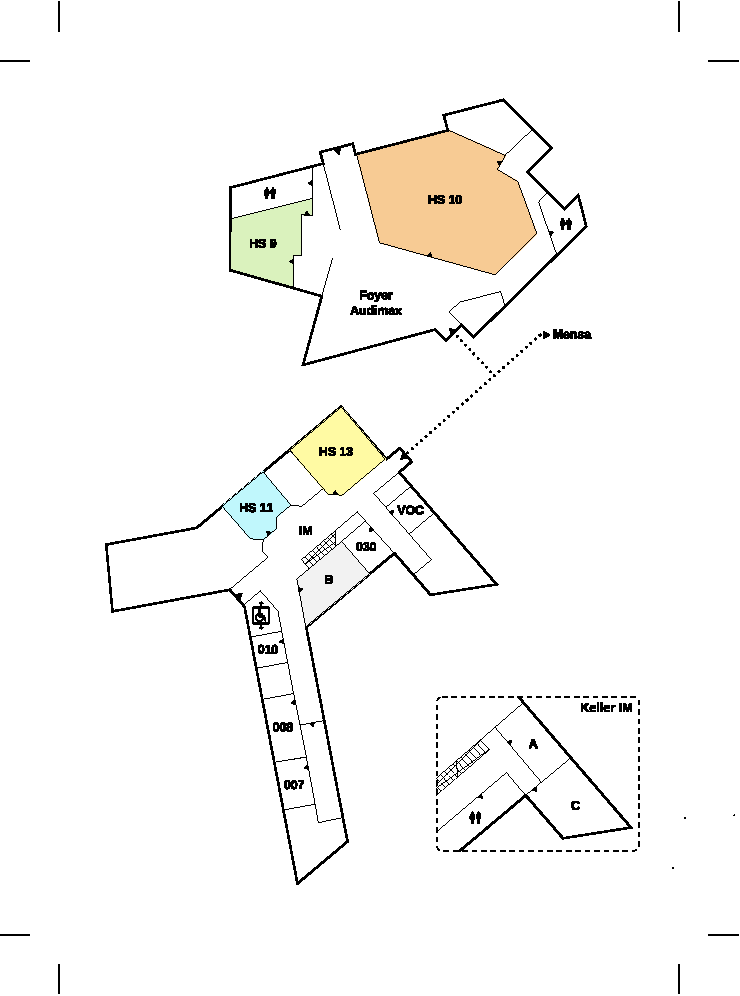
\includegraphics{wallpaper/raumplan-a6.pdf}%
}]{raumplana6}
\newpairofpagestyles[scrheadings]{raumplan}{}
\AddLayersAtBeginOfPageStyle{raumplan}{raumplana6}
\pagestyle{raumplan}
\null
\label{raumplan-page}


\end{document}
